\mychapter{5}{5. Wyniki} \label{chap:outcomes}

\section{Wstęp}

W celu zbadania działania systemu przeprowadzone zostały następujące pomiary:
\begin{itemize}
\item pomiar czasu wykonania programu w zależności od liczby samochodów na skrzyżowaniu 
\item pomiar ilości kroków czasowych po których wszystkie samochody opuszczą skrzyżowania w zależności od liczby samochodów na skrzyżowaniu
\end{itemize}

Pomiary zostały wykonane na dwóch sieciach dróg:
\begin{itemize}
\item skrzyżowanie ze sobą ośmiu dróg
\item skrzyżowanie ze sobą czterech dróg
\end{itemize}

Drogi na obydwu sieciach mają rozmiar 24. Reprezentacja graficzna skrzyżowań jest przedstawiona na rysunku \ref{both-crossroads} z przykładowymi rozmieszczeniami pojazdów.
\begin{figure}[H]
    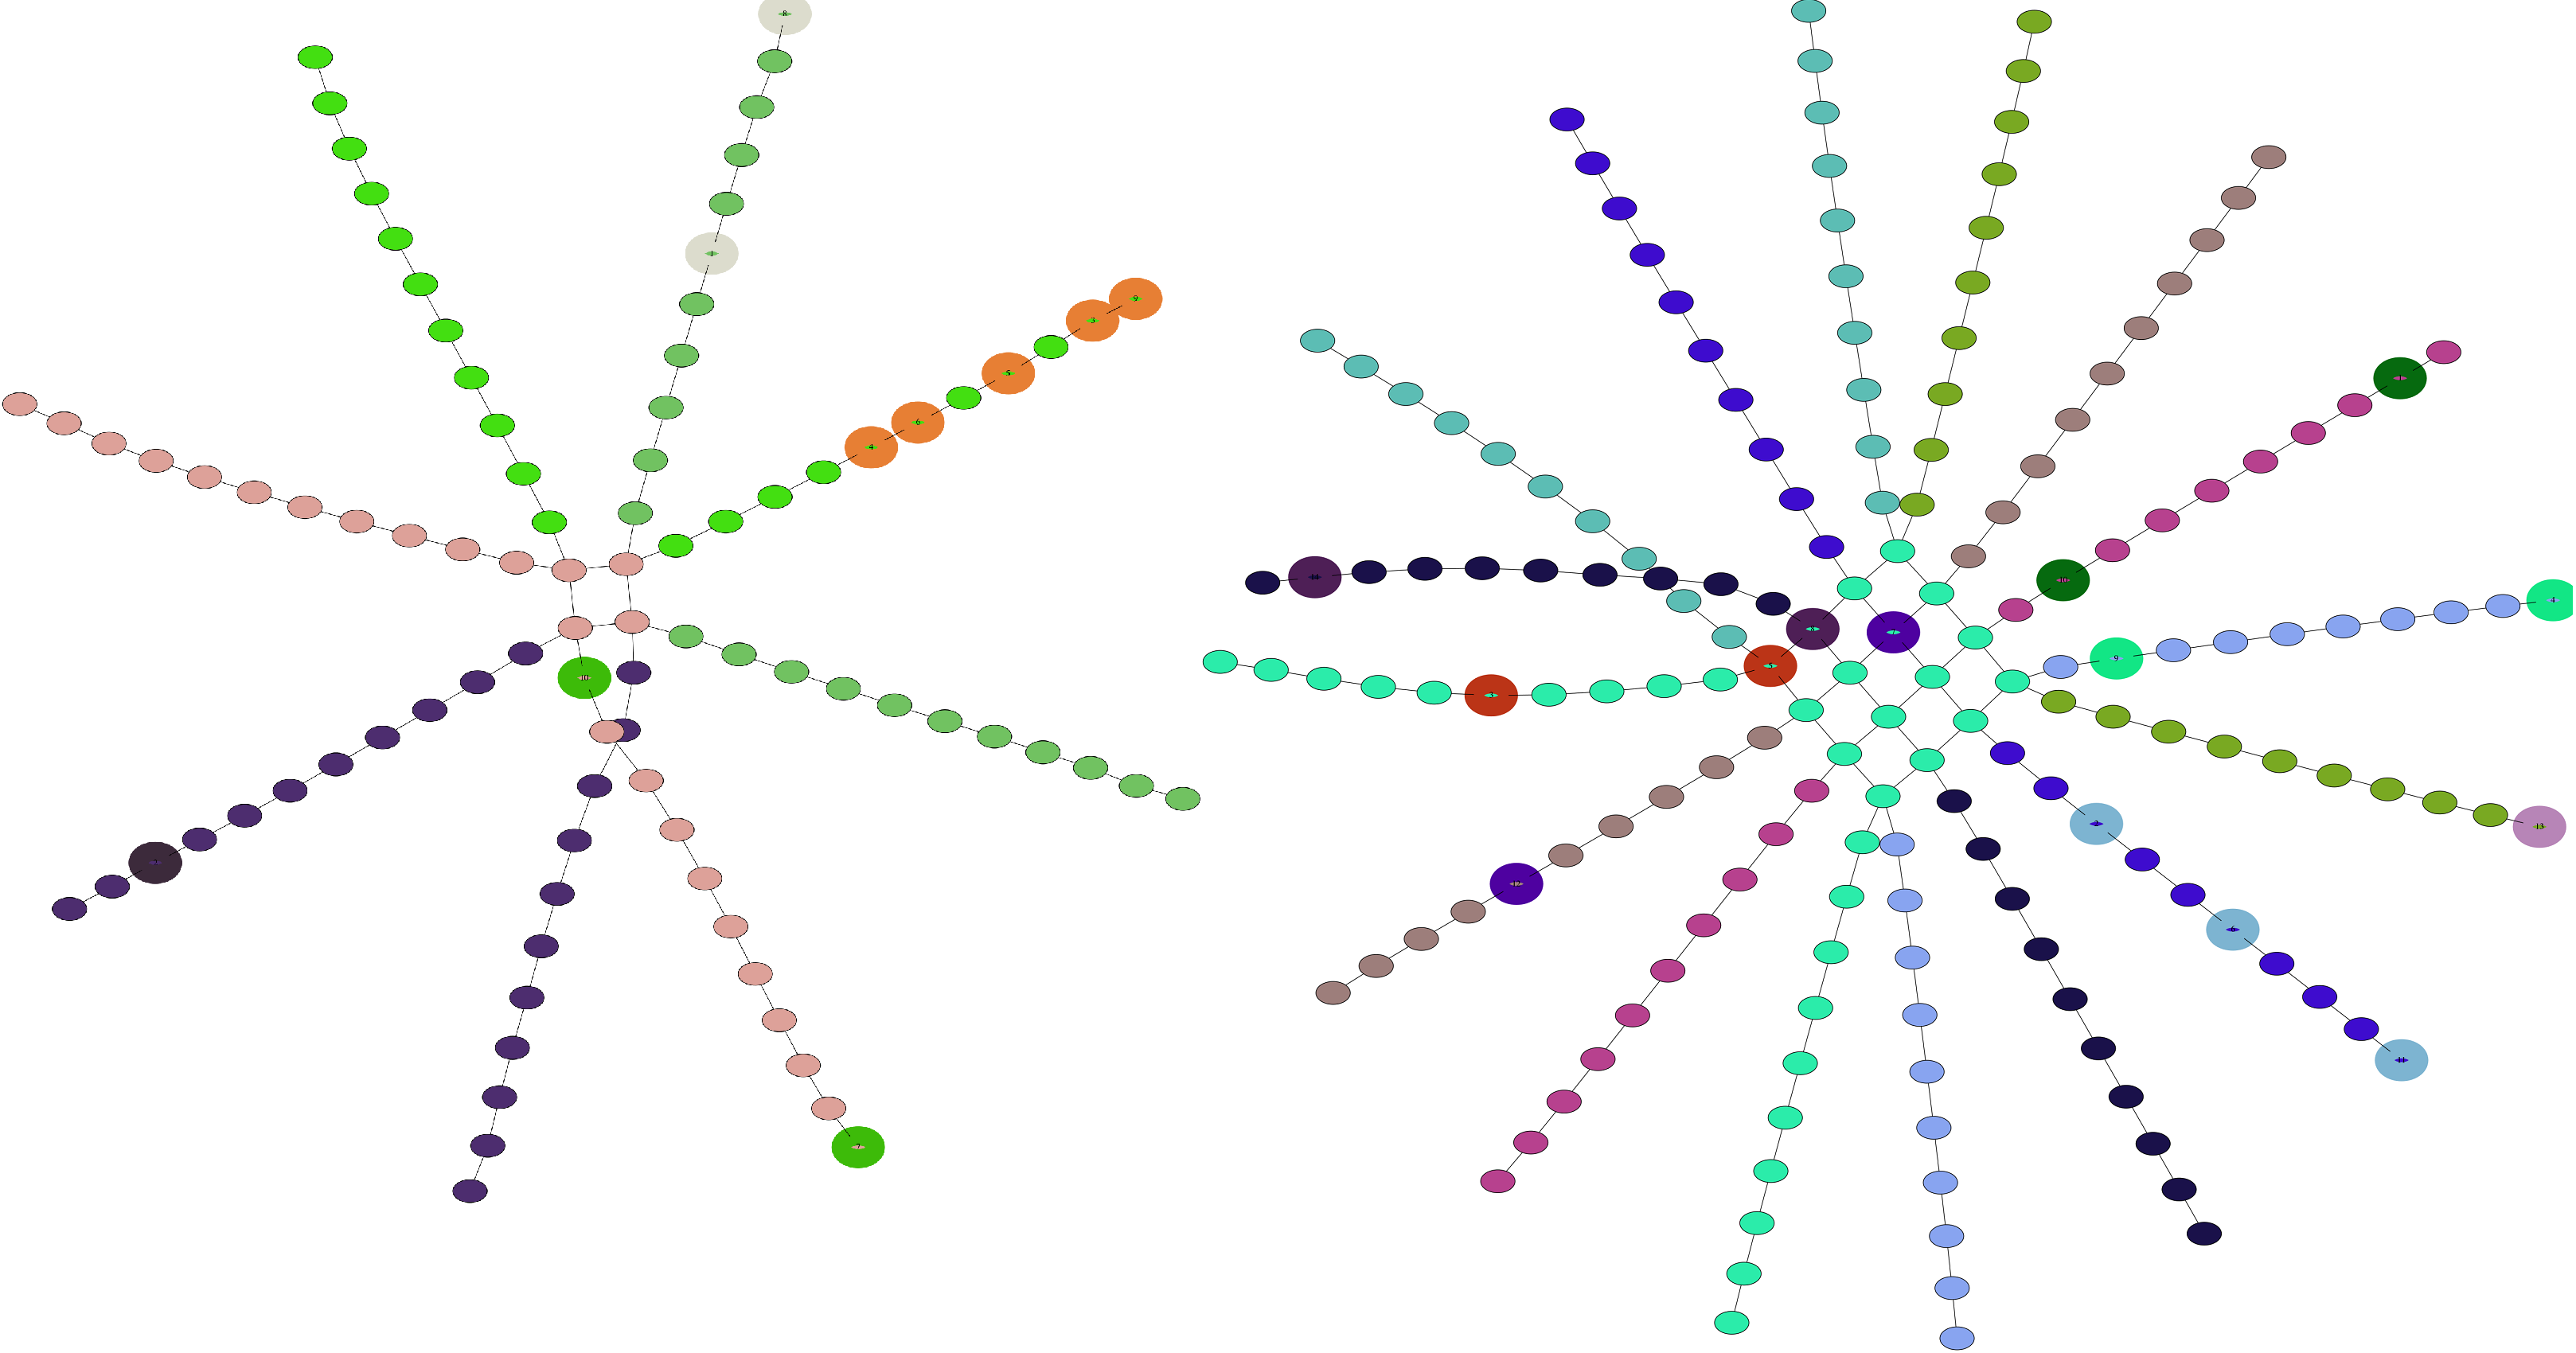
\includegraphics[width=1.0\textwidth]{2_crossroads.png}
  \caption{Skrzyżowanie czterech oraz ośmiu dróg}
  \label{both-crossroads}
\end{figure}

Pomiary zostały przeprowadzone dla następującej liczby samochodów \{2, 4, 6, 8, 10, 12\}. Dla każdej liczby samochodów wygenerowane losowo zostało 30 położeń pojazdów przy założeniu, że żaden z pojazdów nie startuje za ostatnim skrzyżowaniem. Skrypt losujący przyjmuje jako dane wejściowe opis sieci skrzyżowań, liczbę samochodów oraz liczbę stanów startowych do wygenerowania.
\newline
\newline
Pomiary zostały wykonane na następującym sprzęcie:
\begin{itemize}
\item Procesor: Intel(R) Core(TM) i7-4700MQ CPU @ 2.40GHz
\item Liczba rdzeni procesora: 2 - Obliczenia zostały wykonane na jednym wątku
\item 16 GB pamięci RAM
\end{itemize}

\section{Wyniki pomiarów dla skrzyżowania czterech dróg}

Zgodnie z wcześniej opisanymi założeniami dla skrzyżowania czterech dróg program został uruchomiony 30 razy dla samochodów ze zbioru \{2, 4, 6, 8, 10, 12\} co razem daje 180 uruchomień.
\newline
\newline
Wykresy przedstawiające wyniki na skrzyżowaniu czterech dróg zaprezentowane są na rysunkach \ref{execution_time_10_cars_4_roads}, \ref{execution_time_12_cars_4_roads} oraz \ref{four-roads-crossroads-timesteps}
\begin{figure}[H]
  \centering
  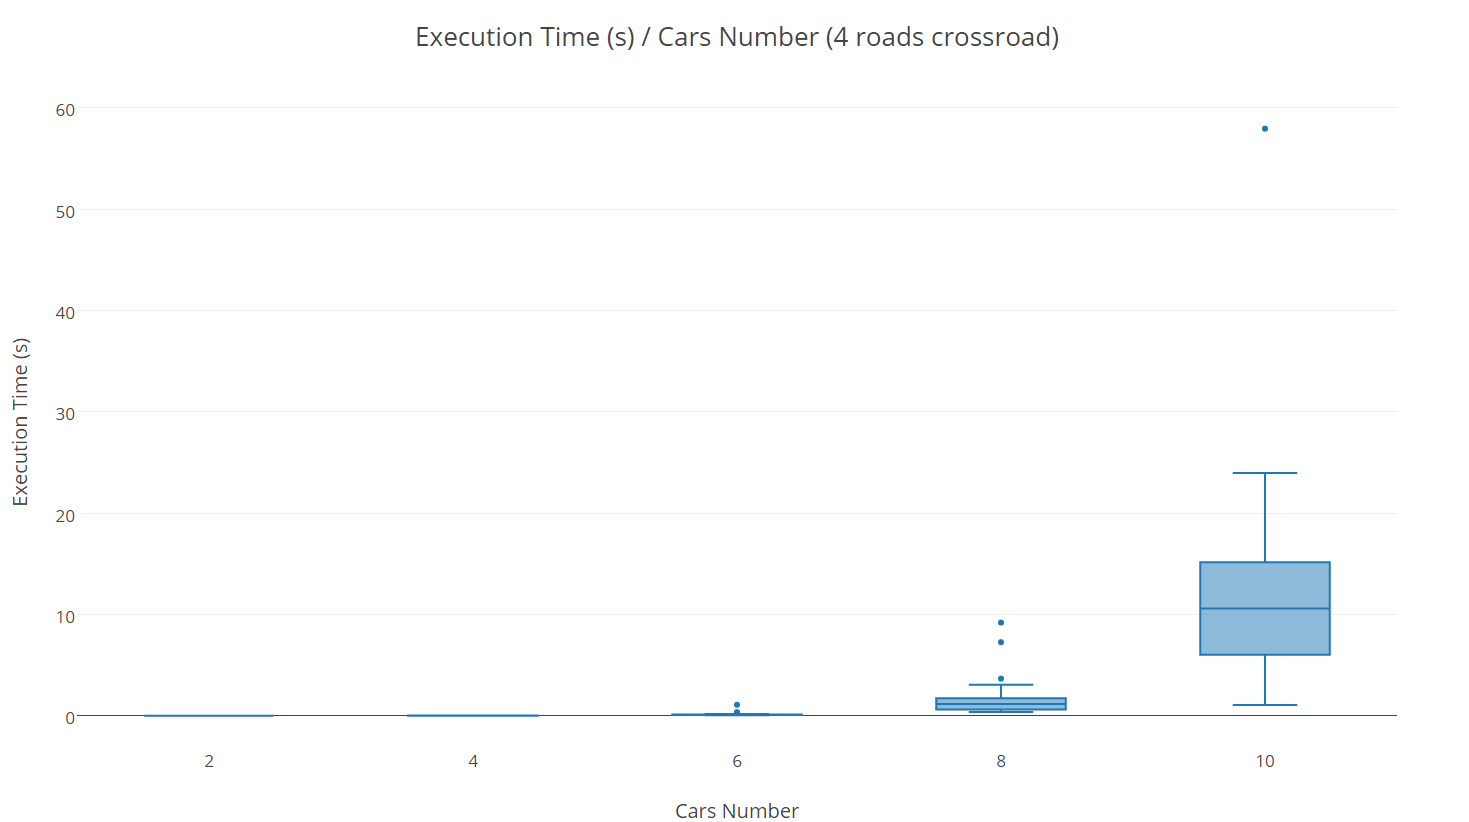
\includegraphics[width=0.8\textwidth]{execution_time_10_cars_4_roads.png}
  \caption{Wykres zależności czasu wykonania programu od liczby pojazdów (dla 2-10 pojazdów)}
  \label{execution_time_10_cars_4_roads}
\end{figure}
\begin{figure}[H]
  \centering
  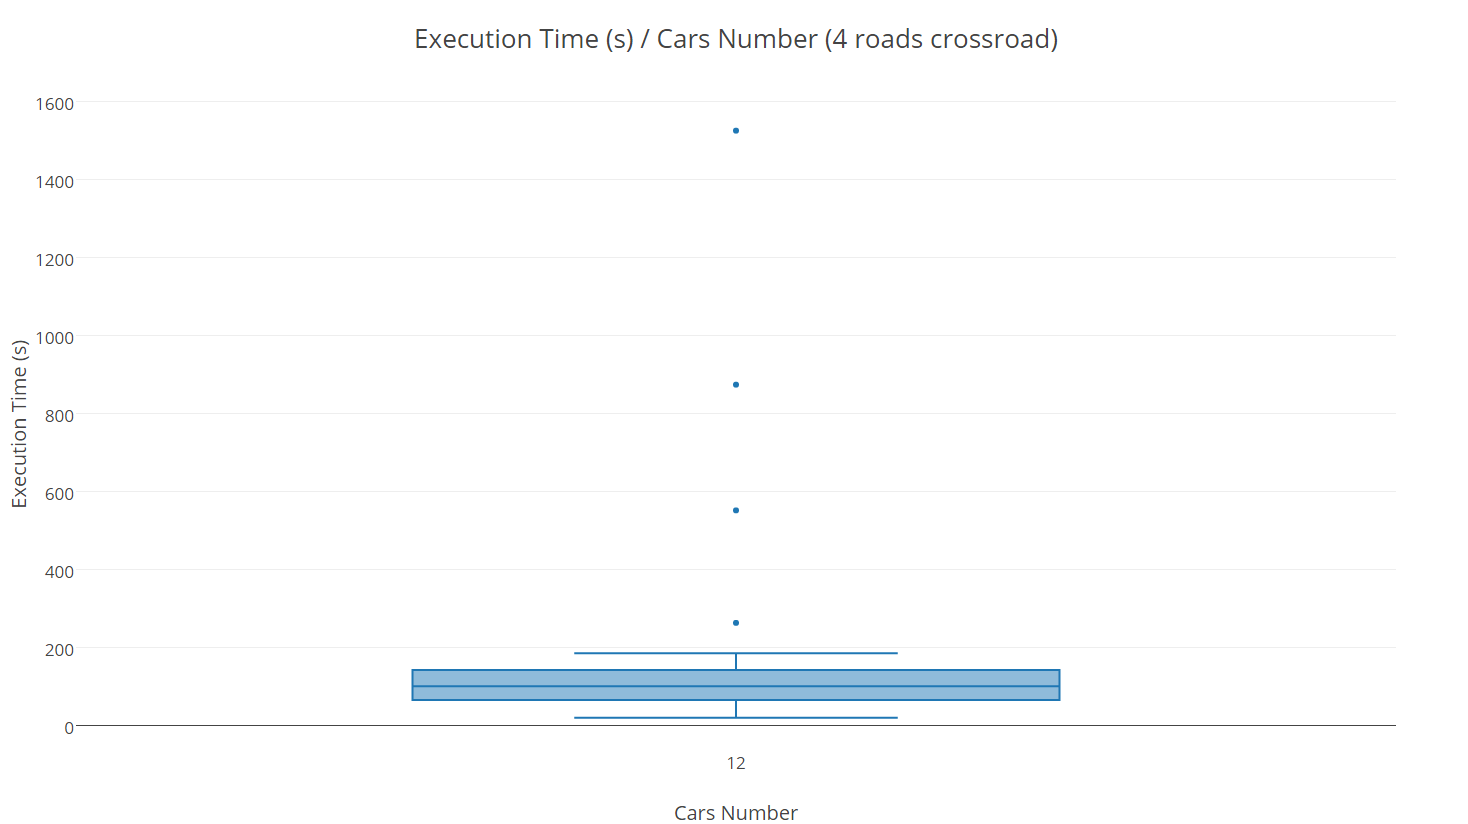
\includegraphics[width=0.8\textwidth]{execution_time_12_cars_4_roads.png}
  \caption{Wykres zależności czasu wykonania programu od liczby pojazdów (dla 12 pojazdów)}
  \label{execution_time_12_cars_4_roads}
\end{figure}
\begin{figure}[H]
  \centering
  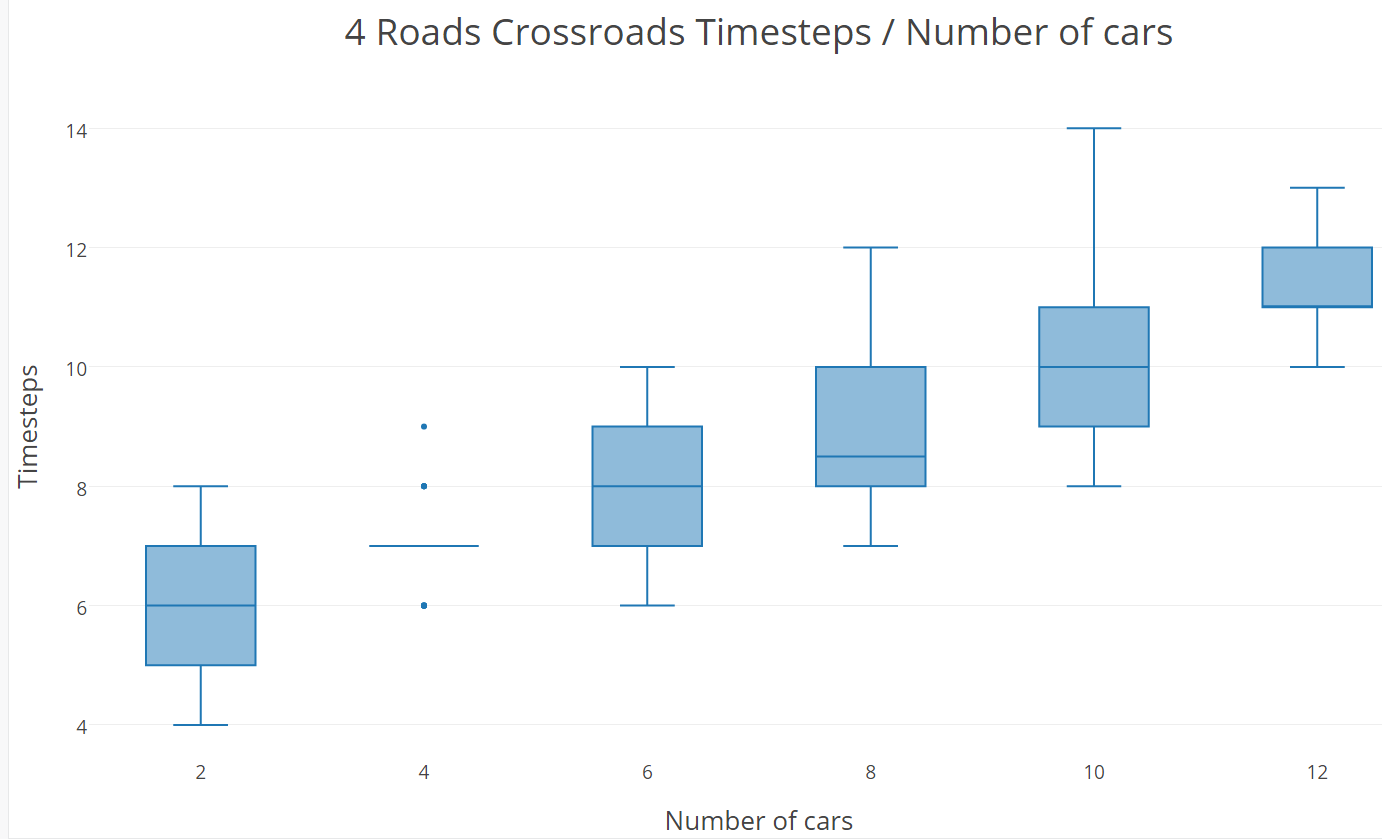
\includegraphics[width=0.8\textwidth]{4_roads_timesteps_2.png}
  \caption{Wykres zależności kroków czasowych od liczby pojazdów}
  \label{four-roads-crossroads-timesteps}
\end{figure}

\section{Wyniki pomiarów dla skrzyżowania ośmiu dróg}

Dla skrzyżowania ośmiu dróg też zostało przeprowadzone 180 uruchomień.
\newline
\newline
Wykresy przedstawiające wyniki na skrzyżowaniu ośmiu dróg zaprezentowane są na rysunkach \ref{execution_time_10_cars_8_roads}, \ref{execution_time_12_cars_8_roads} oraz \ref{eight-roads-crossroads-timesteps}
\begin{figure}[H]
  \centering
  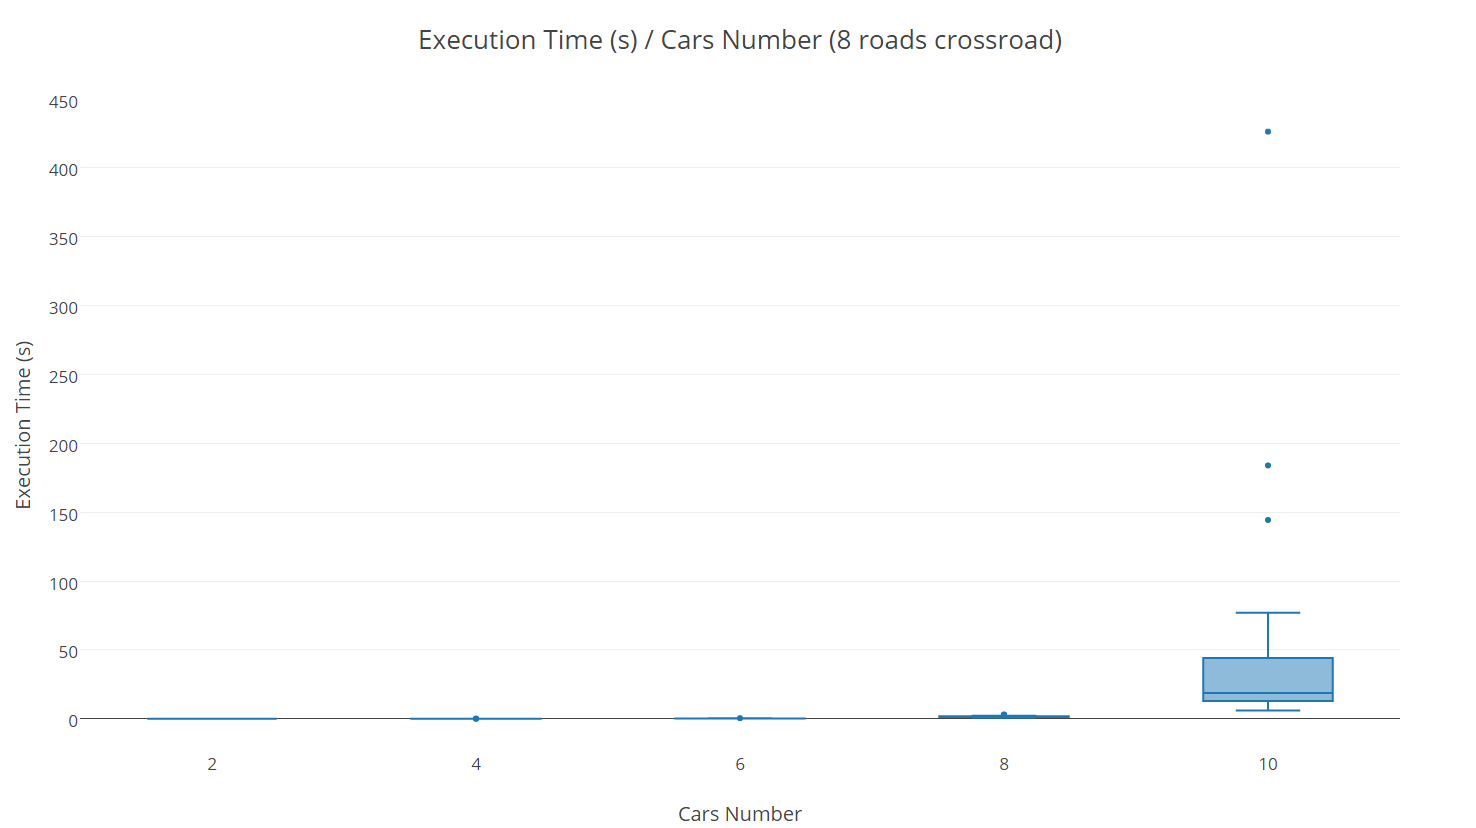
\includegraphics[width=0.8\textwidth]{execution_time_10_cars_8_roads.png}
  \caption{wykres zależności czasu wykonania programu od liczby pojazdów (dla 2-10 pojazdów)}
  \label{execution_time_10_cars_8_roads}
\end{figure}
\begin{figure}[H]
  \centering
  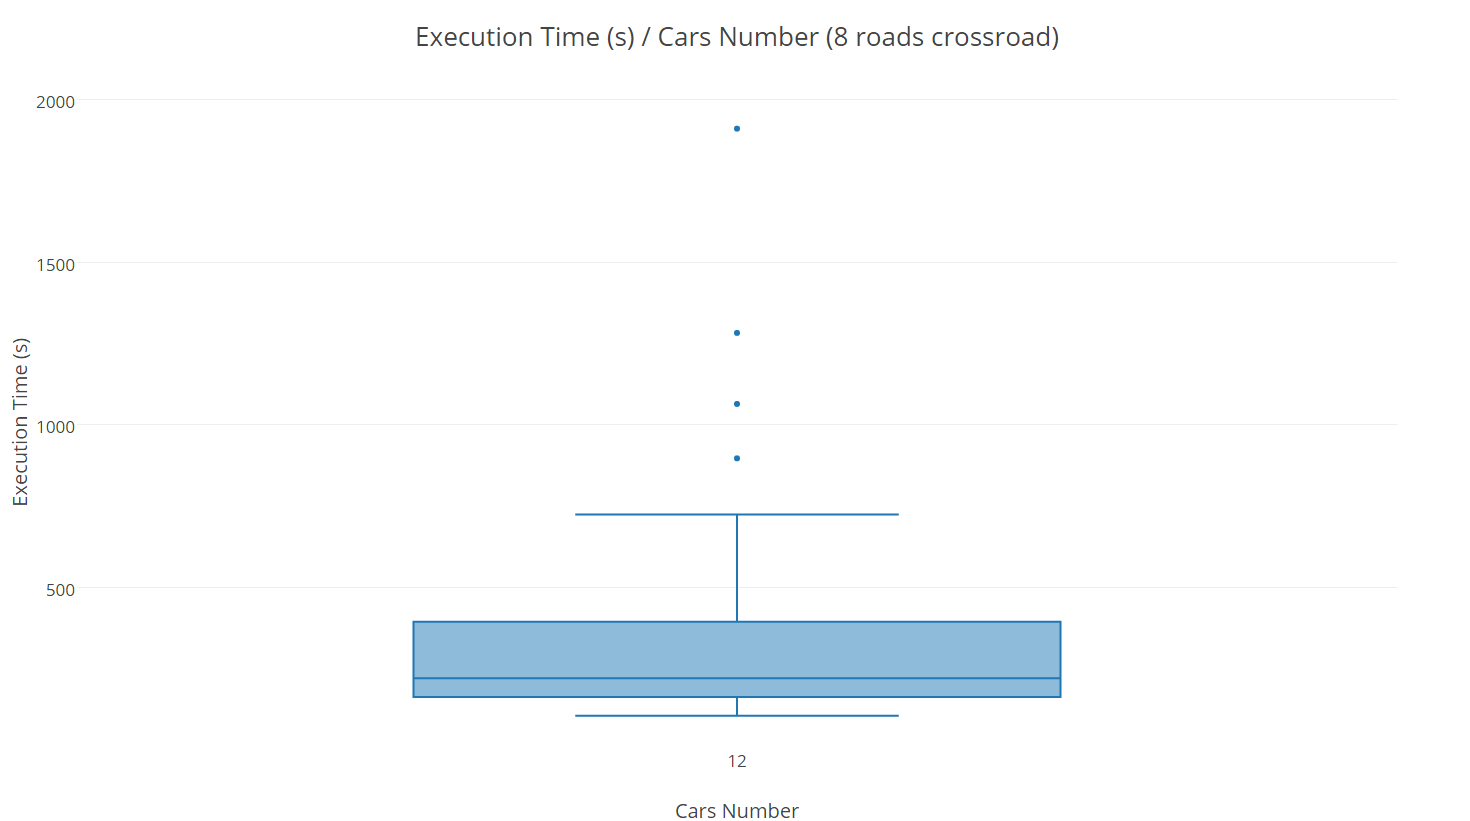
\includegraphics[width=0.8\textwidth]{execution_time_12_cars_8_roads.png}
  \caption{wykres zależności czasu wykonania programu od liczby pojazdów (dla 12 pojazdów)}
  \label{execution_time_12_cars_8_roads}
\end{figure}
\begin{figure}[H]
  \centering
  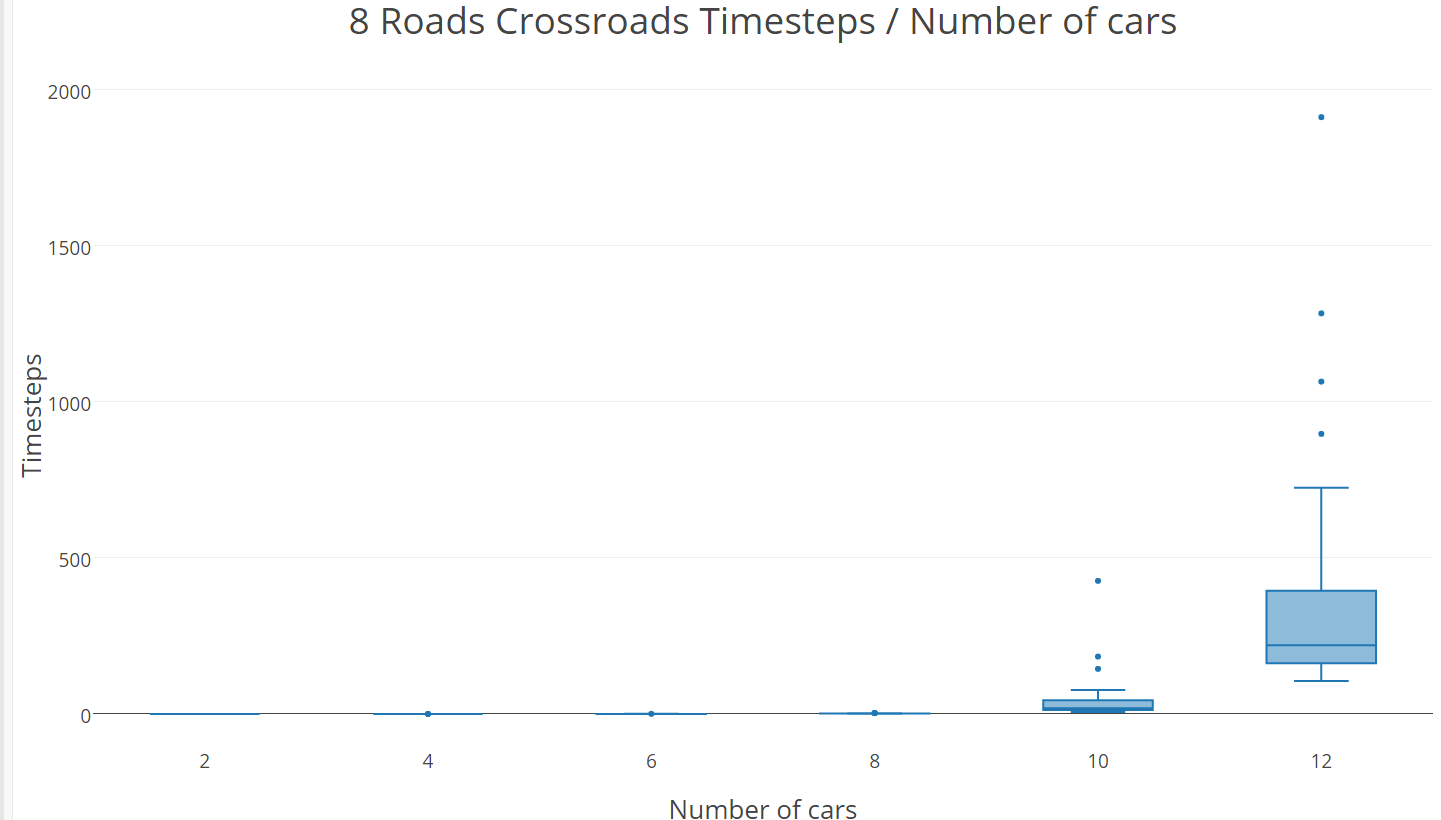
\includegraphics[width=0.8\textwidth]{8_roads_timesteps_2.png}
  \caption{Wykres zależności kroków czasowych od liczby pojazdów}
  \label{eight-roads-crossroads-timesteps}
\end{figure}

\section{Wnioski z pomiarów na skrzyżowaniach czterech i ośmiu dróg}

Wykresy zależności czasu wykonywania względem liczby samochodów na skrzyżowaniu pokazują ograniczenie metody względem liczby samochodów. Jak widać, czas wykonania rośnie ekspotencjalnie względem liczby samochodów. Dla 12 pojazdów czas wykonania przekracza nawet 25 min. Dla sieci skrzyżowań, na której jest 12 lub więcej samochodów użycie metody jest zbyt czasochłonne.
\newline
\indent
Wykresy zależności liczby kroków czasowych po których wszystkie samochody opuszczą skrzyżowania pokazują, że liczba kroków czasowych rośnie liniowo względem liczby pojazdów. 
\newline
\indent
Liczba kroków czasowych na skrzyżowaniu ośmiu dróg jest mniejsza niż na skrzyżowaniu czterech dróg. Spowodowane jest to tym, że na skrzyżowaniu czterech dróg auta stoją jedno za drugim na pasach, bez wolnej przestrzeni przed sobą. W porównaniu do skrzyżowaniu ośmiu dróg, auta mogą swobodnie poruszać się na pasie i częściej wymijają kolizję na skrzyżowaniu.

\section{Prawdopodobieństwo kolizji}

W celu przetestowania bezpieczeństwa rozwiązania zostały przeprowadzone pomiary prawdopodobieństwa kolizji w przypadku pomyłek pojazdów. Pomyłka polega na niezastosowaniu się pojazdu do planu. W rozwiązaniu zaimplementowane zostało symulowanie kolizji pojazdów z określonym prawdopodobieństwem. W każdym kroku czasowym każdy z pojazdów myli się z podanym wcześniej prawdopodobieństwem. Wynikiem pomiarów jest zależność prawdopodobieństwa kolizji od prawdopodobieństwa pomyłki. Zmierzone zostało prawdopodobieństwo kolizji w razie pomyłek pojazdów z następującymi prawdopodobieństwami \{0.001, 0.005, 0.01\}
\newline
\indent
W obliczeniach pod uwagę wzięty został także parametr bezpieczeństwa. Pomiary zostały wykonane dla skrzyżowania 8 dróg, na których znajdowało się 10 pojazdów. Program uruchomiony został 30 razy dla parametru bezpieczeństwa równego 0 oraz 30 razy dla parametru bezpieczeństwa równego 1, aby pokazać jakie bezpieczeństwo gwarantuje użycie parametru bezpieczeństwa.
\newline
\newline
Wyniki z parametrem bezpieczeństwa równym 0 zareprezentowane są w tabeli \ref{firstCollision}
\begin{table}[H]
    \centering
    \begin{tabular}{|c|c|c|c|}
      \hline 
      Prawdopodobieństwo pomyłki & 0.001 & 0.005 & 0.01 \\
      \hline
      Prawdopodobieństwo kolizji & 0.2 & 0.27 & 0.54 \\
      \hline
    \end{tabular} 
    \caption{Prawdopodobieństwo kolizji z parametrem bezpieczeństwa równym 0}
    \label{firstCollision}
\end{table}
\noindent
Wyniki z parametrem bezpieczeństwa równym 1 zareprezentowane są w tabeli \ref{secondCollision}
\begin{table}[H]
    \centering
    \begin{tabular}{|c|c|c|c|}
      \hline 
      Prawdopodobieństwo pomyłki & 0.001 & 0.005 & 0.01 \\
      \hline
      Prawdopodobieństwo kolizji & 0 & 0 & 0.24 \\
      \hline
    \end{tabular} 
    \caption{Prawdopodobieństwo kolizji z parametrem bezpieczeństwa równym 0}
    \label{secondCollision}
\end{table}
Jak pokazują wyniki w tabelach \ref{firstCollision}, \ref{secondCollision} parametr bezpieczeństwa niweluje prawdopodobieństwo kolizji dla małych prawdopodobieństw (0.001, 0.005) pomyłki do zera. Dla prawdopodobieństwa pomyłki równego 0.01, parametr bezpieczeństwa nie zapobiega całkowicie kolizjom - w przeprowadzonych badaniach zmniejszył je o 30\%.

\section{Porównanie wyników z rozwiązaniem ze światłami drogowymi}

W celu zweryfikowania szybkości podejścia z wykorzystaniem algorytmu A*, pomiary zostały porównane z rozwiązaniem polegającym na optymalizacji świateł drogowych przedstawionym w pracy [TUTAJ CYTAT PRACY SEBASTIANA]. Porównywane rozwiązanie także jest oparte o kroki czasowe. Drogi także są dyskretne, mierzone w odcinach, a prędkość też mierzona jest w ilości odcinków drogi na krok czasowy.
\newline
\indent
Rozwiązania różnią się modelami danych, które reprezentują skrzyżowania oraz znajdujące się na nich pojazdy. W jednym rozwiązaniu położenie i droga aut jest określona za pomocą grafu oraz wierzchołków grafu, przez które auta będą przechodzić. W opisywanym w tej pracy rozwiązaniu drogi są opisywane poprzez ich rozmiar oraz przecięcia z innymi drogami. Położenia samochodów natomiast poprzez numer drogi oraz numer odcinka drogi na której się znajdują.
\newline
\indent
Wykonując pomiary uzgodnione zostały wspólne warunki w obu rozwiązaniach tak, aby można było porównać rozwiązania. Porównywane są kroki czasowe, po których wszystkie auta opuszczą skrzyżowanie. Wspólne warunki są następujące:
\begin{itemize}
\item Maksymalna prędkość samochodów wynosi 4 odcinki drogi na krok czasowy
\item Wartości przyspieszeń pojazdów są następujące: \{-1, 0, 1\}
\item Losowane położenia pojazdów w celu wykonania 30 pomiarów są wykonywane w taki sposób, aby żaden pojazd nie znajdował się za skrzyżowaniem
\item Rozwiązanie kończy obliczenia, kiedy wszystkie pojazdy znajdą się za skrzyżowaniem
\item Pomiary zostały wykonane na skrzyżowaniu ośmiu dróg dla następujących liczb pojazdów \{2, 4, 6, 8, 10 ,12\}
\item Drogi mają rozmiar 24
\end{itemize}
Wykres z wynikami pokazany jest na rysunku \ref{comparison}
\begin{figure}[H]
  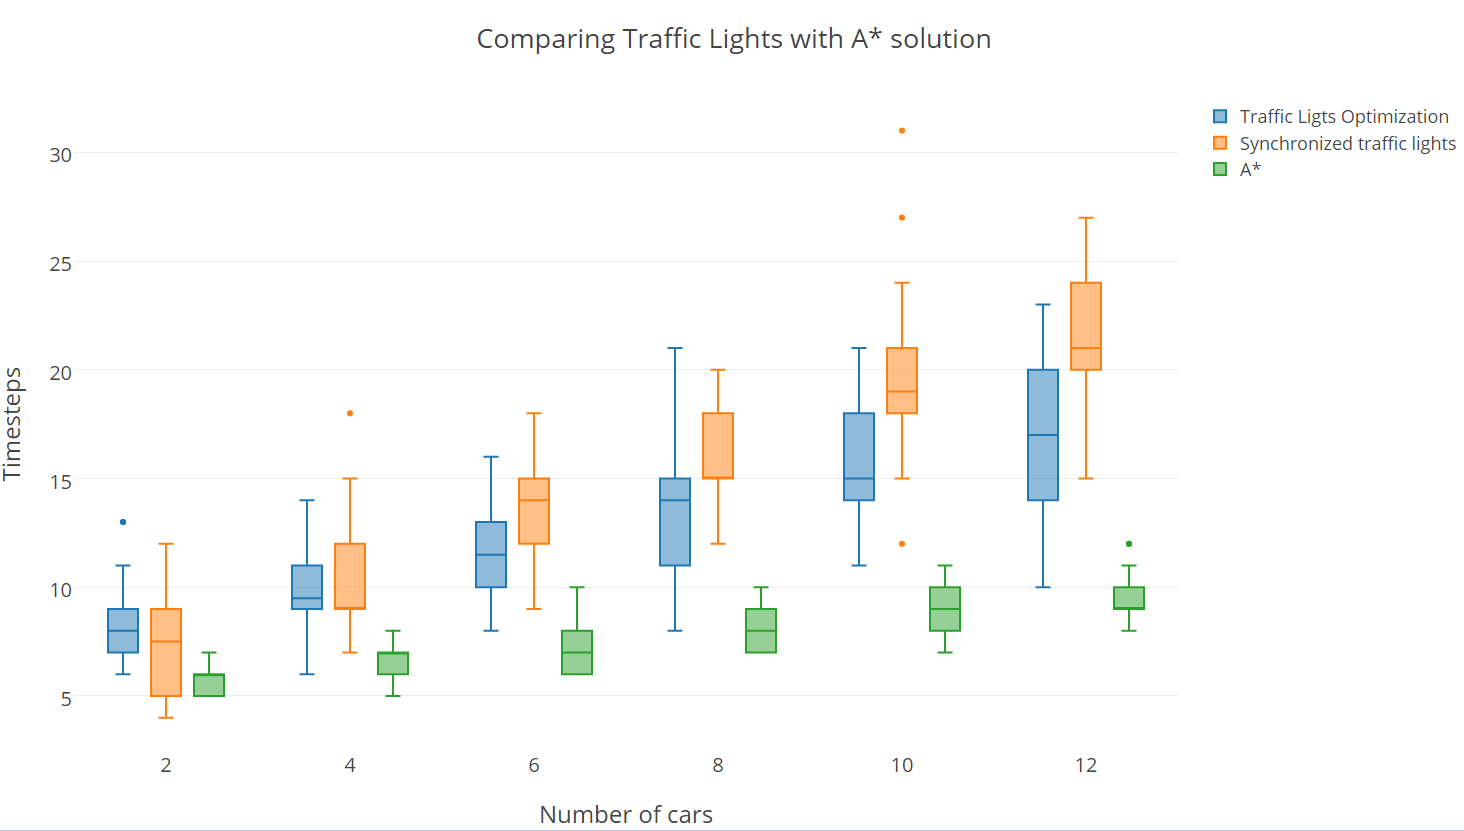
\includegraphics[width=1.0\textwidth]{8_roads_comparison_2.png}
  \caption{Porównanie rozwiązania z użyciem A* ze światłami drogowymi na skrzyżowaniu ośmiu dróg}
  \label{comparison}
\end{figure}
Rozwiązanie z wykorzystaniem algorytmu A* daje lepsze wyniki na tle rozwiązania ze światłami sekwencyjnymi oraz z ich optymalizacjami. Zgodnie z przedstawioną tezą, przepustowość na skrzyżowaniach jest lepsza w rozwiązaniu A* w porównaniu do świateł. Rozwiązanie korzystające z algorytmu A* dla 12 pojazdów nie przekracza 15 kroków czasowych. Dla świateł zoptymalizowanych przekracza 20 kroków czasowych, a dla świateł sekwencyjnych przekracza 25 kroków czasowych. Przedstawione w pracy rozwiązanie zaoszczędza 5-10 kroków na jednym skrzyżowaniu dla 12 pojazdów. Wykorzystując metodę dla dużej sieci skrzyżowań, można zaoszczędzić dużo czasu.
